
% !TEX root = main.tex
\section{Problem Model}
\label{sec:framework}

In this section, we formalize our problem, followed by a restatement based on concept based inference.

\subsection{Problem Statement}
For a given pair of entity, we formalize the problem of explaining the relationship between them as finding the attribute with a probability ranking.
More formally, given an entity pair $ \langle e_1, e_2 \rangle $, we want to find:
\begin{equation}
\argmax_a P(a|\langle e_1,e_2 \rangle),
\end{equation}
where $P(a| \langle e_1, e_2 \rangle )$ is the probability that $a$ is an attribute between two entities.
For example, for entity pair \at{<Bill Gates, Microsoft>}, \at{FounderOf, BoardOf} are among the most probable relations.
However relation like \at{KeyPeopleOf} is not that typical. 

%We give notations used in this paper in Table~\ref{tab:notation}.

\subsection{Concept-based Inference}
Thus our problem is reduced to the estimation of $P(a| \langle e_1, e_2 \rangle )$.
The direct estimation is difficult since no such samples are available.
We resort to the concepts of entities to bridge the inference from entity pair to their attribute.
The rationality comes from the observation that {\it it is the concept determines the relationship between entities}. For example, \at{<Washington, USA>} can be best explained by \at{CapitalOf} attribute, which essentially is determined by the concept pair \at{<Capital City, Country>}.
In other words, a relationship can be considered as generated by corresponding concept pairs.
The entity pairs that belong to the same concept pairs share the same relationship explanation.
Continue the previous example, \at{<Beijing, China>} is clearly another example of entity pairs belonging to \at{<Capital, Country>} that can be explained by the \at{CapitalOf} attribute.

Using concept pairs as intermediate random variables, our problem can be restated as:
\begin{equation}
\label{eq:target}
\argmax_a \sum_{c_i\in C_1 , c_j \in C_2 }P(a|\langle c_{i},c_{j}\rangle)\times P(\langle c_{i},c_{j}\rangle|\langle e_{1},e_{2}\rangle),
\end{equation}
where $P(a|\langle c_{1},c_{2}\rangle)$ is the probability that attribute $a$ is relationship between the concept pair
and $P(\langle c_{i},c_{j}\rangle |\langle e_{1},e_{2}\rangle)$ is the probability that $\langle c_1, c_2\rangle$ is the concept pair of $ \langle e_1, e_2 \rangle $.
$P(a| \langle c_{1},c_{2} \rangle )$ can also be regarded as the {\it typicality} of attribute $a$ given the concept pair.
For the same concept pair, some attribute is more typical than another one.
For concept pair \at{<artist, country>}, the attribute \ac{hometown} is more typical than \ac{education}.
For a given entity pair, some concept pair is better to characterize the concept of the entity pair than others.
As example,  for \at{<apple, Steve Jobs>},  \at{<company, entrepreneur>} deserves a higher probability than \at{<food, name>}.
$P( \langle c_{i},c_{j} \rangle | \langle e_{1},e_{2} \rangle )$ can also be considered as the typicality of the concept pair for the given entity pair.


Another benefit of concept-level estimation is that it can reduce the computation cost.
In general, the number of concept pairs is significantly less than that of entity pairs.

\section{Joint Conceptualization}
In this section, we present our solution to estimate $ P(\langle c_1,c_2 \rangle | \langle e_1,e_2\rangle) $.
Our basic idea is considering the conceptualization of $e_1$ and $e_2$ jointly instead of independently.
By joint conceptualization, we derive a new optimization objective function.


\subsection{Estimation of $P(\langle c_1,c_2\rangle | \langle e_1,e_2\rangle)$ }
A straightforward estimation of $P( \langle c_{1},c_{2} \rangle | \langle e_{1},e_{2} \rangle )$ is as Eq~\ref{eq:naive} when we assume that the choice of concept for $e_1$ is independent of that for $e_2$.
\begin{equation}
\label{eq:naive}
\begin{split}
P(\langle c_{1},c_{2}\rangle |\langle e_{1},e_{2} \rangle) = P(c_1|e_1) P(c_2|e_2)
\end{split}
\end{equation} The rationality is that the typicality of a concept pair can be quantified as the product of their respective typicality of each concept given its corresponding entity.
However, the assumption does not always hold as shown in Example~\ref{exa:jc}. Hence, we need to introduce a factor $\alpha(c_1,c_2)$ into Eq.~\ref{eq:target_expand2_jr} to quantify {\it how likely that the two concepts are the appropriate concepts of the attribute}. Thus, we have the following improved estimation:
\begin{equation}
\label{eq:target_expand2_jr}
\begin{split}
P(\langle c_{1},c_{2}\rangle |\langle e_{1},e_{2} \rangle) = \alpha(c_1,c_2)  P(c_1|e_1)  P(c_2|e_2)
\end{split}
\end{equation}


One simple estimation of $\alpha(c_1,c_2)$ is using the prior probability of $\langle c_1, c_2\rangle$, i.e., $P(\langle c_1,c_2\rangle)$ (see Eq.~\ref{eq:rel_jdp}).
\begin{equation}\label{eq:rel_jdp}
  \alpha(c_1,c_2) = P(\langle c_1, c_2\rangle)
\end{equation}
This is reasonable since the true concept pair for an entity pair in general has a larger probability than
a false concept pair.

Using Bayesian rules, $P(a| \langle c_{1},c_{2} \rangle )$ can be restated by the following equation:
\begin{equation}
\label{eq:target_expand1}
P(a|\langle c_{1},c_{2} \rangle)= \frac{ P(\langle c_{1},c_{2}\rangle|a)P(a) }{ P(\langle c_{1},c_{2}\rangle) }
\end{equation},
where $P(a)$ is probability to observe an entity pair with attribute $a$.
Thus the objective function is reduced to Eq.~\ref{eq:simple_obj} when Eq.~\ref{eq:rel_jdp} holds.
\begin{equation}
\label{eq:simple_obj}
 \argmax_a \sum_{c_i\in C_1, c_j\in C_2} P(\langle c_{i},c_{j}\rangle |a) P(a) P(c_i|e_1) P(c_j|e_2)
\end{equation}




\nop{
\subsection{Target Expand}
Given, Eq~\ref{eq:target}, the estimation of $P(a| \langle e_1,e_2 \rangle )$ boils down to 2 parts:
\begin{enumerate}
\item $P(a| \langle c_{1},c_{2} \rangle )$:  the typicality of an attribute for a concept pair.
\item $P( \langle c_{i},c_{j} \rangle | \langle e_{1},e_{2} \rangle )$:  the typicality of the concept pair for an entity pair.
\end{enumerate}

Using Bayesian rules, $P(a| \langle c_{1},c_{2} \rangle )$ can be restated in Eq.\ref{eq:target_expand1}:
\begin{equation}
\label{eq:target_expand1}
\begin{split}
P(a|\langle c_{1},c_{2} \rangle) &= \frac{ P(\langle c_{1},c_{2}\rangle|a)\times P(a) }{ P(\langle c_{1},c_{2}\rangle) }
%&=\frac{ p((c_{1},c_{2})|a)\times P(a) }{ \sum{P( (c_{1},c_{2})|a^* )\times P(a^*)   } },
\end{split}
\end{equation},
where $P(a)$ is probability to observe an entity pair with attribute $a$.
}

\subsection{Solution Framework}
Now we are ready to present our framework. The main framework is illustrated in Figure~\ref{fig:framework}, which consists of two major components: the {\it online computation} and {\it offline training}. We refer to our system as \ac{Entity Relation Finder(ERF)}.
ERF takes an entity pair as input and find its most plausible relation as the result.
As a preprocessing step, we first directly lookup the attribute for the query entity pair from DBpedia.
If DBpedia has SPO triples connecting the entity pair, we direct return the predicate as the answer.
Otherwise, the procedure goes into the online computation component.
The online component calculates $ P(a|  \langle e_1,e_2 \rangle  )$ for each candidate attribute in $A$ (the set of all attributes) by Eq.~\ref{eq:simple_obj} and return the maximal one as the answer attribute. To compute Eq.~\ref{eq:simple_obj}, we need to compute $P(c_1,c_2|a)$, $P(a)$, $P(c_1|e_1)$ and $P(c_2|e_2)$. 

We compute $P(c_1|e_1)$ and $P(c_2|e_2)$ on demand instead of materializing them. Because we only conceptualize an entity into its head concept and the conditional probability of head concept cannot be carefully recaculated. In general, a materialization suffers from quadratic complexity, which is unaffordable when we have millions of entities. We will elaborate it later in head-aware conceptualization section.
In the offline part, we compute $P(c_1,c_2|a)$ and $P(a)$ by leveraging the SPO triples in DBpedia and isA relationships in Probase. We elaborate their computation detail in the next section.





\begin{figure}[!ht]
\centering
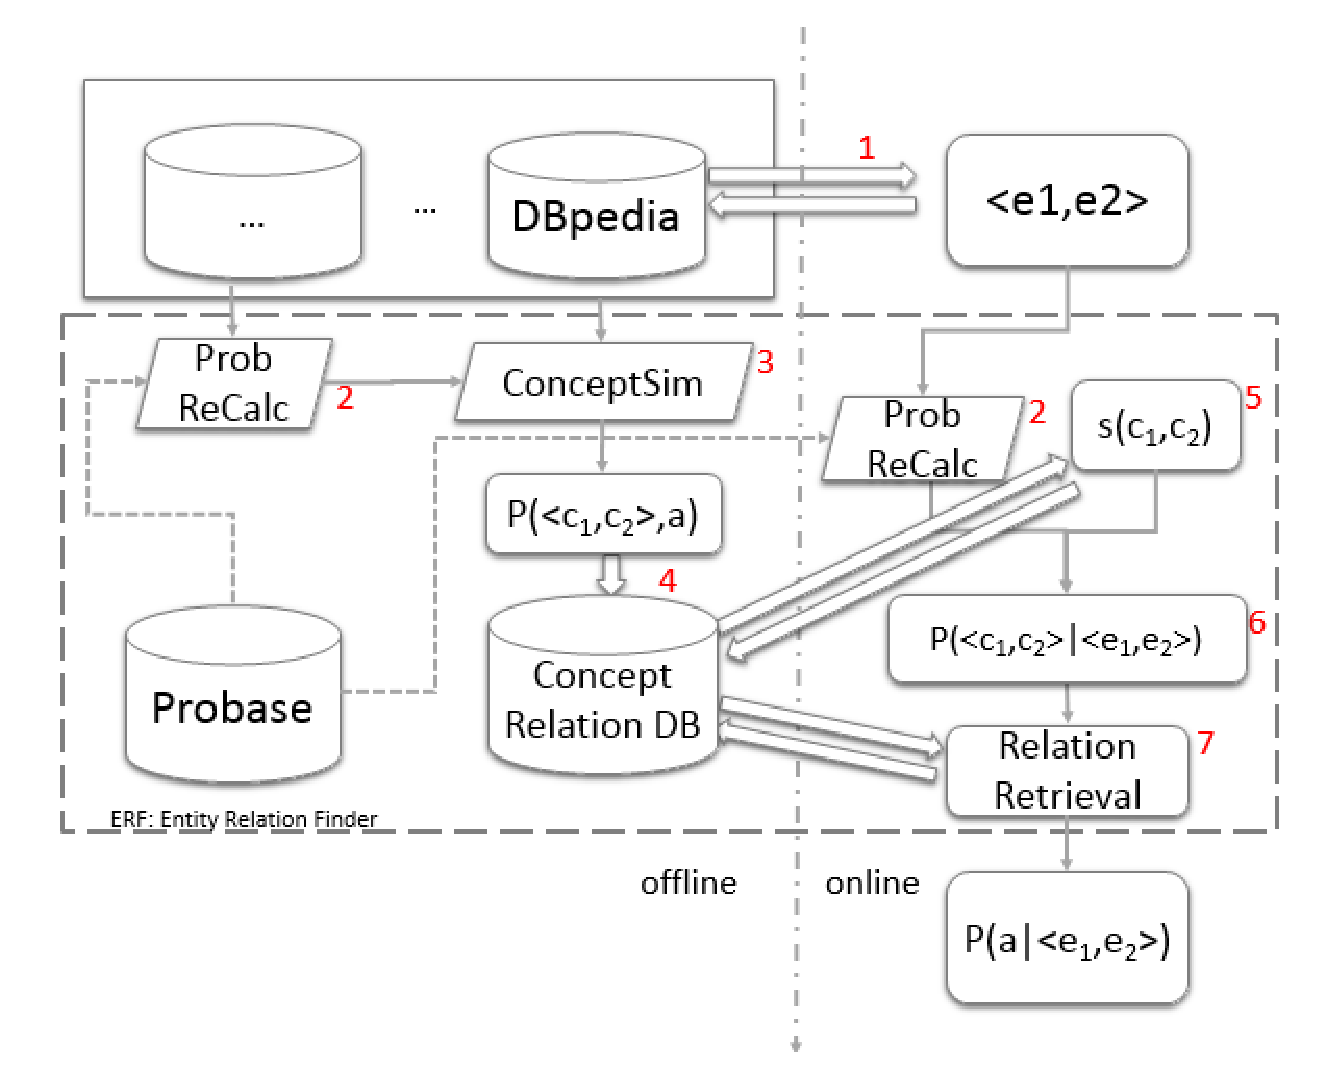
\epsfig{file=resources/framework.eps,width=0.5\columnwidth,height=0.25\columnwidth}
\caption{System Framework of ERF}
\label{fig:framework}
\vspace{-6mm}
\end{figure}


\nop{
In the online part, we first directly lookup the attribute for the query entity pair from DBpedia.
If DBpedia has no the exact the SPO triples connecting the entity pair, we In $step 2$, the concepts of the entities in knowledge bases are calculated(i.e. $P(c_i|e_i)$ in Eq.~\ref{eq:target_expand2_jr}).
The detailed process in in
$Step 3$ is the training process, $P( \langle c1,c2 \rangle ,a)$ is calculated for every attribute $a$ in Eq.~\ref{eq:pccga}.
The result is then stored in Concept Relation DB in $step 4$.

In  $step 1$, when a query entity pair comes, knowledge bases such as DBpedia are looked up and the exact relationship, if exists, is answered in the first place.
If nothing is found in $step 1$, the process will go into the ERF solution.

We first conceptualize the 2 entities in $step 2$.
The concept similarity score in Eq.~\ref{eq:target_expand2_jr}) is retrieved from the Concept Relation DB in $4$.
%\ref{eq:pcca}
So far we get everything for calculating Eq.~\ref{eq:target_expand2_jr}).
Then in $step 7$ we query the concept relation database and get the relation between concept pairs, specifically, $P(a| \langle c_1,c_2 \rangle )$ in Eq.~\ref{eq:target_expand1}.
Finally, we achieve the final object by combining all these together to infer $\argmax P(a| \langle e_1,e_2 \rangle )$ from Eq.~\ref{eq:target_expand_all}.
We return the the attribute owning the maximal score as the explanation for the relationship between the entity pair.

When no direct edges are found, we use the shortest path on the concept attribute graph to find the middle concepts, then the problem automatically reduced to relation explanation of several pairs of entities, discussing which is beyond the coverage of this paper.
}


%\paragraph{Paper Orgnization}
%The rest of the paper is organized as follows, Section~\ref{sec:conceptualization} describe how to derive $P(c|e)$ leveraging the \xch{basicness} of concept, Section~\ref{sec:fafa} is devoted to the offline calculation of $JD(c_1,c_2)$ and $P((c_{1},c_{2})|a)$.
%\renewcommand\baselinestretch{-6}\selectfont
\renewcommand{\arraystretch}{-2}
%
%\begin{table}[htbp]
%  \centering
%     \small
%  \caption{Notation Table}
%    \footnotesize
%
%    \begin{tabular}{|ll|ll|}
%    \hline
%    notation                            &  meaning                            & notation                            &  meaning  \\
%    \hline
%    $n(\cdot)$                          &  count of                            & $e_i$                               &  entity  \\
%    $h(\cdot)$                          &  head of                             & $c_i$                               &  concept  \\
%    $a$                                 &  attribute                          & $c_l$                               &  long concept  \\
%    $\bar{C}$                           &  head concept set                  & $c_h$                               &  head concept  \\
%    $\langle e_1,e_2\rangle$            &  entity pair                        & $\langle c_1,c_2\rangle$            &  concept pair \\
%    $\alpha(\cdot,\cdot)$               &  joint factor                       & $T_k$                               & \parbox{0.26\columnwidth}{ set of E$A$E tuple with $a_k$ as $A$} \\
%    \parbox{0.15\columnwidth}{\scriptsize $P(a|\langle c_{1},c_{2}\rangle)$ }  &  \parbox{0.24\columnwidth}{ the typicality of an attribute for a concept pair. }& \parbox{0.23\columnwidth}{\scriptsize $P(\langle  c_{i},c_{j}\rangle|\langle e_{1},e_{2}\rangle)$} & \parbox{0.26\columnwidth}{ the typicality of the concept pair for an entity pair} \\
%    \hline
%
%    \end{tabular}%
%
%  \label{tab:notation}%
%  \vspace{-6mm}
%\end{table}%
%
%\renewcommand{\arraystretch}{1}

%First,we do conceptualization.
%
%Next,Judge whether the 2 entities are conceptually same
%
%Then, there are 2 cases of the CanBeExplained function:
%
%\begin{itemize}
%\item Explain 2 conceptually similar entity
%
%\begin{table}[htbp]
%  \centering
%  \caption{conceptually similar entity}
%    \begin{tabular}{rr}
%    \toprule
%    entity & concept \\
%    \midrule
%    Steve jobs & Person \\
%    Bill Gates & Person \\
%    \bottomrule
%    \end{tabular}%
%  \label{tab:addlabel}%
%\end{table}%
%
%
%\item Explain 2 conceptually different entity
%% Table generated by Excel2LaTeX from sheet 'Sheet1'
%\begin{table}[htbp]
%  \centering
%  \caption{Add caption}
%    \begin{tabular}{rr}
%    \toprule
%    entity & concept \\
%    \midrule
%    Mona Lisa & Painting \\
%    Renaissance & Period \\
%    \bottomrule
%    \end{tabular}%
%  \label{tab:addlabel}%
%\end{table}%
%
%Note that the concept here are not unique.
%
%\end{itemize}
%
%
%Last, We rank all the explanations in each step.
%
%
%

\section{Collective Conceptualization (Offline Learning)}
In this section, we elaborate how we estimate $P(a)$ and $P( \langle c_{1},c_{2} \rangle |a)$ from knowledge bases, which is the major task in the offline learning component. As we have claimed, our major idea is collectively conceptualize multiple EAE instances instead conceptualizing each instance independently.
% We also introduce computation of $P(a)$ is another important part of the offline component.


\subsection{Collective Conceptualization ($P( \langle c_{1},c_{2} \rangle |a)$) }
For a certain attribute $a_k$, there are many entity pairs connected by the attribute in DBpedia.
We use SPO triples in DBPedia to compute the probability.
%We use these entity-attribute-entity instances to estimate the conditional probability of a concept pair given an attribute. 
The key of the computation is to assign a larger value for the true concepts pairs than false concept pairs.
To achieve this, we aggregate the support from all entity pairs.
The aggregated score can help identify the true concept pair due to the following
obvious facts:
\begin{enumerate}
\item \emph{A false concept pairs are only supported by quite a few
entity pairs that have the attribute.}
\item \emph{A true concept pairs in general are supported by most entity pairs of the attribute.}
\end{enumerate}

More formally, let $ \langle e_i, a_k, e_j \rangle $ be a SPO triple in DBPedia.
%The triple means that entity $e_i$ has a attribute $a_k$ with value or object as $e_j$.
%We only consider the SPO triples with O as entity, this attributes such as \at{height,year} are removed in the first place. 
Let $T_k=\{\langle e_i, a_k, e_j \rangle\}$ be all the triples in DBpedia with attribute as $a_k$.
$P( \langle c_1, c_2 \rangle |a_k)$ is estimated as follows:
\begin{equation}
P(\langle c_1, c_2\rangle|a_k)= \frac{1}{|T_k|}\sum_{  (e_{i},a_k,e_{j})\in T_k } P(c_1|e_{i})P(c_2|e_{j})
\label{eq:pccga}
\end{equation}
It is not difficult to prove that $0\leq P( \langle c_1, c_2 \rangle |a_k)\leq 1$ and their sum over all concept pairs equals to 1.
Hence $P( \langle c_1, c_2 \rangle |a_k)$ is a probability estimation.

\begin{example}[Calculating $P( \langle {c_h}_{1},{c_h}_{2} \rangle  |a)$]
\label{exa:pggga}
Figure~\ref{fig:bipartite} shows many entity pairs of attribute \at{FoundedBy}. 
We can see that the false concept such as \at{fruit} supported by only \at{Steve Jobs}.
However, the true concept pair \at{<company, entrepreneur>} are supported by all the three concept pairs. 
By summing up all $P(c_1|e_1)P(c_2|e_2) $ over all entity pairs, the true concept pair \at{<company, entrepreneur>} has the largest score $\mathbf{4.7\times10^{-7}}$ 
Instead, the false one \at{<fruit, entrepreneur>} has $\mathbf{2.4\times10^{-9}}$
\end{example}


\begin{figure}[!htb]
\centering
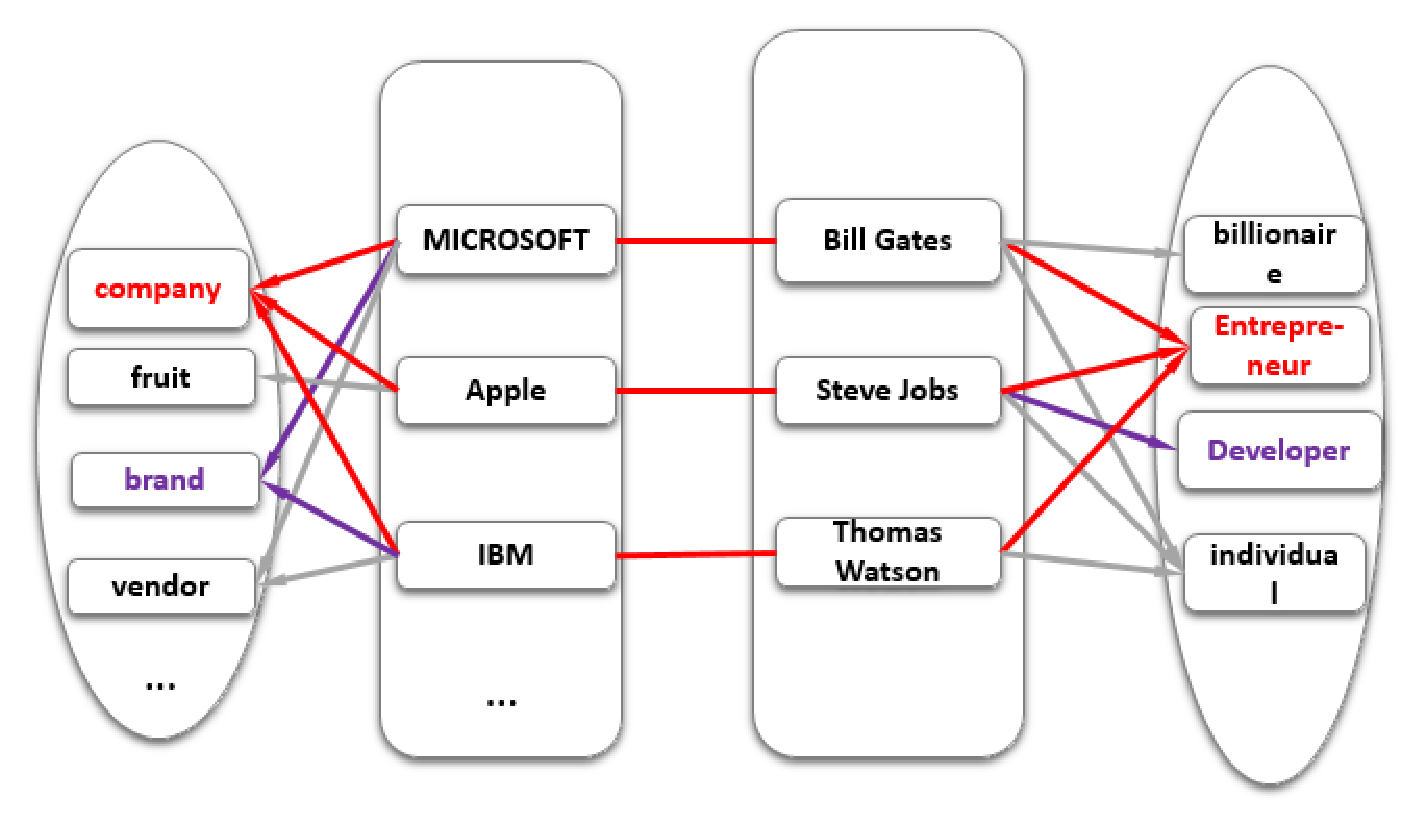
\epsfig{file=resources/ceaec.eps,width=\columnwidth, height=0.4\columnwidth}
\caption{Calculating $P(  \langle {c}_{1},{c}_{2} \rangle  | \term{FoundedBy} )$ }
\label{fig:bipartite}
\vspace{-6mm}
\end{figure}

\nop{
\paragraph{Complexity analysis}

We first analysis the complexity of calculating $P(\langle c_i, c_j \rangle|a_k)$, manifest in Table.~\ref{tab:complexity}. The original one need to calculate $P(\langle c_i, c_j \rangle|a_k)$ for all $c \in C_1,C_2 $,while most of the concepts are, according to the power law, close to zero, which indicates the rationality of pruning.


\begin{table}[htbp]
  \centering
  \caption{Complexity Analysis}
    \begin{tabular}{rr}
    \toprule
    method & complexity \\
    \midrule
    original &  $O(|T_n||C_1||C_2|)$ \\
    topKpruned & $O(|T_n|K^2)$ \\
    \bottomrule
    \end{tabular}%
  \label{tab:complexity}%
\end{table}%
}

\paragraph*{Computation of $P(a)$}
For a given attribute $a$, $P(a)$ can be computed by
\begin{equation}
\label{eq:pa}
P(a)=\frac{n(a)}{\sum_{a_k\in A}{n(a_k)}},
\end{equation}
where $n(a)$ is the count of triples in DBpedia with attribute $a$.



%%% Local Variables:
%%% mode: latex
%%% TeX-master: "main.tex"
%%% End:
